\section{The benchmark, its cleaned export, and the leakage
audit}\label{sec:data}

\paragraph{SWAN-SF and the two substrates.}
SWAN-SF~\cite{angryk2020} partitions solar-active-region time series
into five folds of 60-minute, $60\times24$ multivariate windows over
24 SHARP-style magnetic-flux parameters, with a binary M/X-class
flare label on every window. The community mostly consumes its
\emph{cleaned} export~\cite{eskandari2024}: under-sampled negatives,
Tomek-cleaned boundaries, TimeGAN-augmented positives, imputed
values, and per-partition normalisation --- a pre-balanced substrate
(48.9\% training prevalence) whose natural-prevalence test
partitions carry 1.31--1.88\% positives. This study evaluates on
both substrates: the cleaned export as shipped, and a raw substrate
rebuilt in-pipeline from the raw benchmark (the release's imputation
and normalisation reproduced from their published description, every
parameter fitted on training data only, verified against the
released export on the audit-matched windows, series differences
bounded by $5\times10^{-3}$ at float16 storage). The raw substrate
removes the synthetic positives and the $26\times$ prevalence shift
and asks the classical question: can the models learn the natural
distribution at all?

\paragraph{The provenance audit.}
The cleaned export carries no region or event identifiers, so the
audit first aligns every cleaned window to its raw instance. The raw
benchmark (Harvard Dataverse) encodes, per instance, the flare
class, the HARP region identifier, and window timestamps in its
filenames. The matching key is the per-feature argmax/argmin
position along the 60 timesteps --- 48 discrete invariants that
survive any per-feature monotone normalisation and are robust to the
export's imputation noise. A window is accepted as aligned when at
least 28 of 48 invariants agree (borderline cases additionally
require mean per-feature Spearman $\rho \ge 0.70$). On the test
partitions this verifies 98.7--100.0\% of windows with 100.00\% label
agreement; on the training side, label agreement is 99.71\% (161
disagreements, which bound the synthetic-share estimate below).

\paragraph{What the audit found.}
Three structural facts follow. First, the test export of partition
$p$ contains \emph{all} raw instances of $p$; the counts match
exactly on every partition. Second, the training export of $p$ is a
rebalanced \emph{subset of the same instances}: the verified training
pool covers 56{,}005 unique raw instances, every one of which is
also a test instance (56{,}005/56{,}005) --- and every M/X-flaring
test instance (6{,}234 of 6{,}234, 100\% of the minority class) is
in the training pool. Third, 85.7--90.0\% of the training positive
windows are TimeGAN-synthetic (they have no raw counterpart), while
virtually no negative windows are. The release paper prescribes
pairing temporally-preceding training partitions with a later test
partition; a pipeline that instead pools the training exports and
evaluates on the same partitions' test exports --- the default
drift of any naive consumer --- partially measures memorised data,
most severely for the minority class. Because no HARP region spans
two partitions (verified: 0 shared HARPs), a temporally-preceding
fold is automatically instance-, region-, and time-disjoint.

\paragraph{The leakage-free fold.}
All headline comparisons are therefore re-run under the benchmark's
intended protocol: training on the training exports of partitions
1--4 (77{,}865 windows; 65{,}406 train / 12{,}459 validation after a
stratified carve), and a single-pass evaluation on the test export
of partition 5 (75{,}365 windows, natural 1.31\% prevalence). The raw
substrate uses the same partition structure, so its fold is
leakage-free by the same construction. Everything else is frozen:
six Dirichlet-sketched clients, 50 rounds, seed 42, the focal loss
and calibration machinery of Section~\ref{sec:method}.
Figure~\ref{fig:partition} shows the client partition the federated
arms actually train on.

\begin{figure}[t]
\centering
\begin{adjustbox}{max width=0.88\textwidth}
    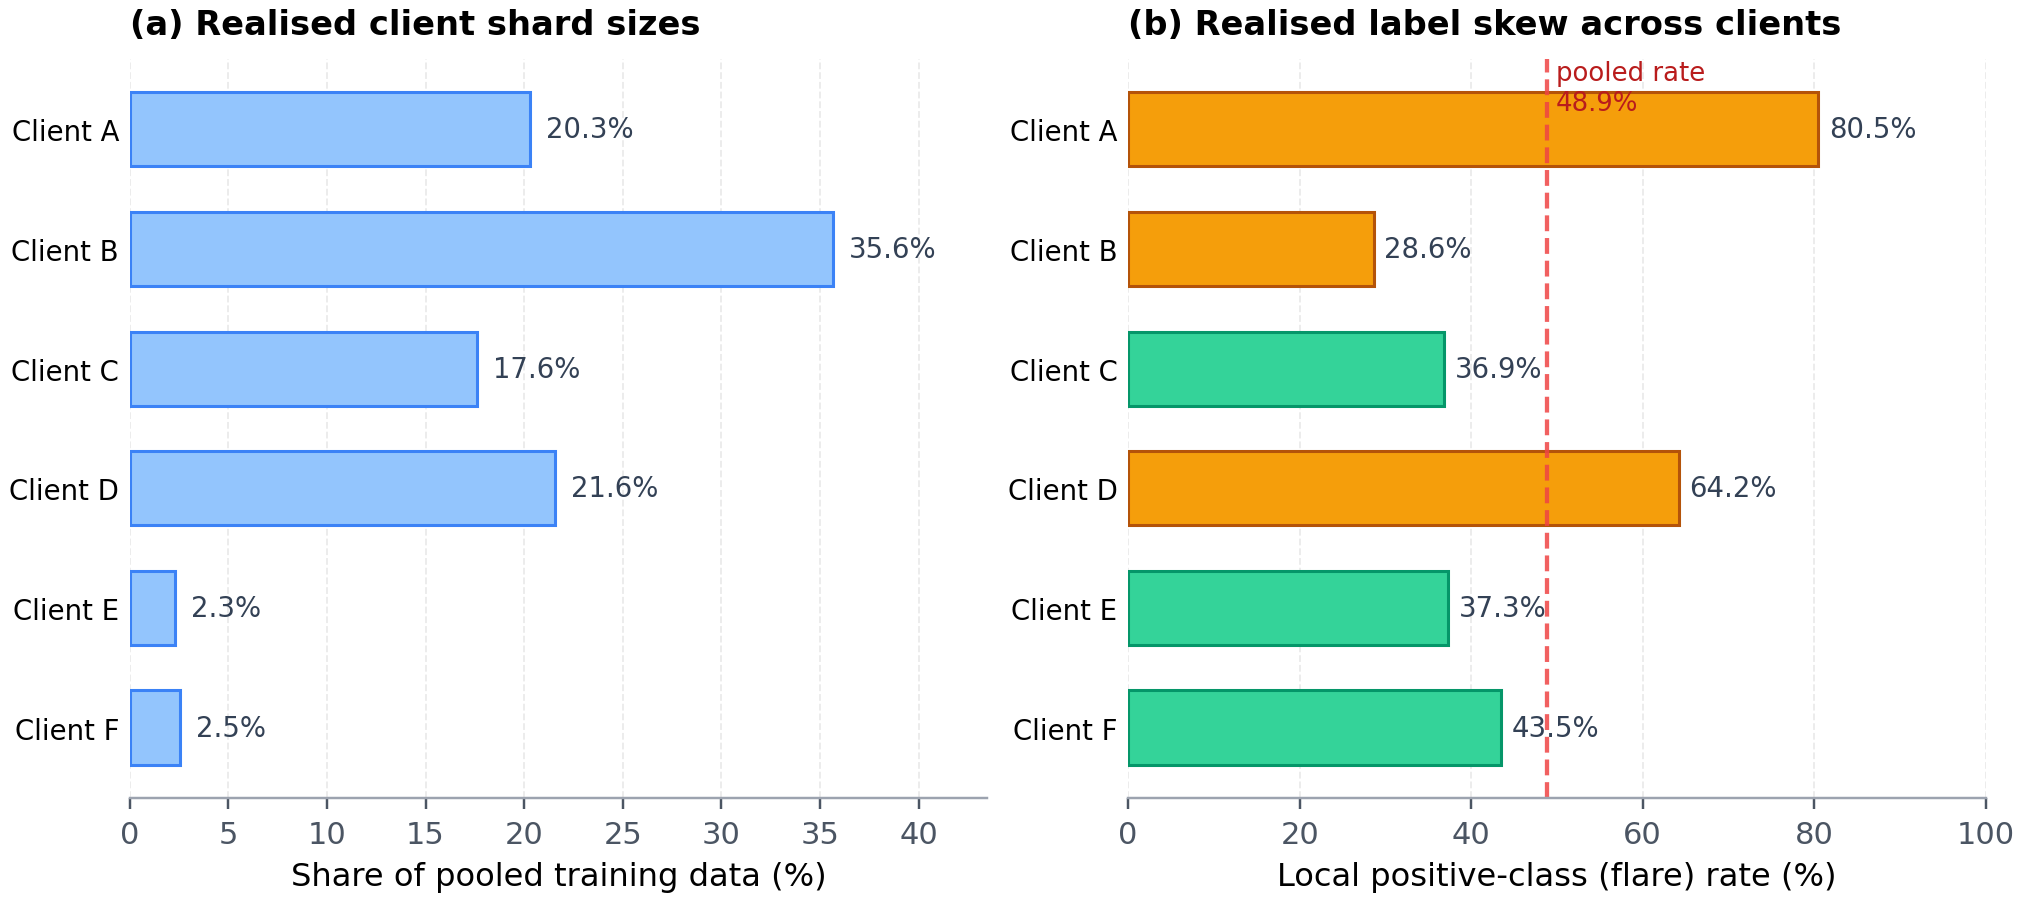
\includegraphics{figures/fig_partition.png}
\end{adjustbox}
\caption{Non-IID partitioning of the pooled training data into six
simulated clients by label-aware Dirichlet sampling (concentration
$\alpha = 1.0$, seed 42). Proportions are read directly from the
frozen run's cached client assignment: the shard sizes and label
skews are the heterogeneity every federated arm of this paper
trains under.}
\label{fig:partition}
\end{figure}
